\chapter{Sistemas de tipos de cambio e integración financiera internacional}

\section{Objetivos del capítulo}

\begin{enumerate}
    \item Introducir una serie de conceptos relacionados con las finanzas internacionales.
    \item Estudiar las diferentes formas de definir los tipos de cambio.
    \item Analizar las ventajas e inconvenientes de un régimen de tipos de cambio fijos frente a un régimen de tipos de cambio flexibles.
    \item Comprender los mecanismos que relacionan internacionalmente las monedas y los tipos de interés.
    \item Explicar las diferentes formas en que se puede medir la integración financiera.
\end{enumerate}

\section{Resumen de contenidos}

\subsection{Los tipos de cambio y los mercados de divisas}

En el comercio internacional la mayoría de transacciones exigen un pago monetario a cambio de la obtención de las mercancías. Sin embargo, por regla general, cada estado emite su propia moneda y, al no existir una moneda internacional común\footnote{No obstante, el dólar, el euro y el yen, junto con la libra esterlina, son monedas muy utilizadas y con dimensión claramente internacional.}, se hace necesario intercambiar unas monedas por otras para pagar las importaciones y cobrar las exportaciones. No obstante, también en el ámbito de las finanzas se producen movimientos internacionales que exigen el uso de moneda extranjera. En concreto, el aumento de la movilidad de capitales derivado de la inversión en activos reales y en activos financieros es otra de las razones que se encuentran detrás de la oferta y la demanda de divisas.

En este contexto, el tipo de cambio bilateral (al que denominaremos, simplemente, tipo de cambio) es la relación de intercambio existente entre dos monedas, es decir, el precio relativo medido en términos de la otra. El método directo (o «Americano») define el tipo de cambio como el número de unidades de moneda nacional necesarias para comprar una unidad de moneda extranjera. Así, para comprar un dólar son necesarios 1,12 \text{€} o para comprar una libra esterlina 1,61 \text{€} y 0,008 \text{€} para comprar un yen. El método indirecto (o «Europeo») define el tipo de cambio como el recíproco del anterior y consiste en el número de unidades de moneda extranjera por unidad de moneda nacional. Así, un euro vale 0,62 libras esterlinas, 0,89 \$ o 125 yenes\footnote{Actualmente, el Banco Central Europeo utiliza esta segunda definición del tipo de cambio. Sin embargo, dado que en los libros de texto de mayor difusión se usa la definición directa, vamos a mantener esta última en nuestra exposición.}. Sin embargo, esta circunstancia no debería suponer ningún problema puesto que, al tratarse de un precio relativo, el valor dependerá de la moneda que se tome como referencia.

Dado que el tipo de cambio de la moneda $k$ respecto a la $s$ ($TC_{ks}$) es el recíproco del tipo de cambio de la moneda $s$ respecto a la $k$ ($TC_{sk}$):

\[
TCE_i = \sum \left[ \left( \frac{TC_{ij}}{TC_{i0}} \right) \times p_j \right] \times 100
\]
\[
TC_{ks} = \frac{1}{TC_{sk}}
\]
\[
TC_{sk} = \frac{1}{TC_{ks}}
\]

debería verificarse lo que se conoce como \textit{condición de consistencia}:

\[
TC_{ks} \times TC_{sk} = 1
\]

Si se define el tipo de cambio según el método directo, se dice que la moneda se \textit{deprecia} cuando aumenta el tipo de cambio, es decir, se hace necesario entregar más unidades de nuestra moneda a cambio de una unidad de moneda extranjera. Por el contrario, se \textit{aprecia} cuando el tipo de cambio disminuye y es posible comprar la moneda extranjera con menos unidades de moneda nacional. En el ejemplo anterior, si el tipo de cambio euro/dólar pasa de ser 1,12 \text{€}/\$ a 1,30 \text{€}/\$ se ha producido una depreciación del euro, puesto que el euro vale menos en términos del dólar. Por el contrario, si el tipo de cambio euro/dólar se reduce hasta 1,05 \text{€}/\$ significaría que se ha apreciado la moneda europea, ya que con menos euros es posible comprar el mismo dólar.

A la hora de hablar de monedas y tipos de cambio, merece también una mención aparte las denominadas \textit{monedas cesta}, que son aquellas monedas expresadas como una media ponderada de una cesta de diversas monedas. Las más conocidas son el Derecho Especial de Giro (DEG), creado por el Fondo Monetario Internacional, y el ECU, o Unidad de Cuenta Europea, que se utilizó durante la vigencia del Sistema Monetario Europeo (SME). Sus valores se expresan, normalmente, en términos de monedas de amplio uso en las transacciones internacionales, como el dólar o libras esterlinas.

Formalmente, si $q_1, q_2, ..., q_n$ son las cantidades de las diversas monedas en una unidad de la moneda cesta, dicha unidad (a la que se puede denominar $N$), se puede definir como:

\[
(q_1, q_2, ..., q_n) = N
\]

Dados los tipos de cambio bilaterales, $TC_{jN}$ se puede definir el valor de $N$ en términos de cualquiera de sus componentes, es decir, lo que sería el tipo de cambio de la moneda $j$ respecto a $N$, de la siguiente forma:

\[
TC_{jN} = \sum q_i TC_{ij}, \quad j = 1, 2, ..., n
\]

Siendo $TC_{jj} = 1$. De esta forma se puede también calcular la ponderación ($p_j$) de cada moneda en la cesta, que se obtiene del cociente entre la cantidad de moneda en la cesta y el valor de la cesta en términos de dicha moneda, es decir:

\[
p_j = \left[ \frac{q_j}{\left( \sum q_i TC_{ij} \right)} \right], \quad j = 1, 2, ..., n
\]

debiendo verificarse que la suma de todas las ponderaciones sea la unidad.

\section{Tipos de cambio cruzados}

Una vez examinadas las relaciones entre los tipos de cambio bilaterales, se puede introducir el concepto de \textit{tipos de cambio cruzados} (o indirectos). El tipo de cambio cruzado de moneda $j$ respecto a la $i$ indica cuántas unidades de la moneda se intercambian indirectamente (es decir, a través de la compra y venta de una tercera moneda, $m$) por una unidad de la moneda $j$. Así, una unidad de la moneda $j$ compra $TC_{jm}$ unidades de la moneda $m$ en el centro financiero $j$; vendiendo esa cantidad de moneda $m$ se puede intercambiar (vendiéndola) en el centro financiero $i$ al tipo de cambio $TC_{mi}$, obteniendo $TC_{jm} \times TC_{mi}$. La condición de consistencia requiere también que coincidan los tipos de cambio directos y cruzados:

\[
TC_{ji} = TC_{jm} \times TC_{mi}
\]

Utilizando el tipo de cambio es posible expresar los precios en la misma moneda. De esta forma, para conocer el precio en euros de una mercancía que vale 5 dólares, por ejemplo, habrá que multiplicar el tipo de cambio por el precio en dólares:

\[ \text{Precio (en dólares)} \times TC \, \text{€}/\$ \]

siendo $TC \, \text{€}/$ el tipo de cambio del euro respecto al dólar. Igualmente, para obtener el precio en dólares:

\[ \frac{\text{Precio (en euros)}}{TC \, \text{€}/\$} \]

Los mercados en los que se intercambian las monedas se denominan \textit{mercados de divisas}. A su vez, las \textit{divisas} son las monedas aceptadas en las transacciones internacionales, dado que no todas las monedas son \textit{convertibles}.

En esos mercados se demandan y se ofrecen las divisas por diversos motivos. Se \textit{demandan divisas} por parte de los importadores, tanto de bienes como de servicios, así como de los exportadores de capitales y los individuos o entidades que envían transferencias al extranjero, como los emigrantes a sus familias. La demanda de divisas será mayor cuanto mayores sean las importaciones y las salidas de capital. Por lo que se refiere a las importaciones, éstas serán mayores cuanto más alta sea la renta nacional y cuanto mayores sean los precios relativos (es decir, precio nacional respecto al precio extranjero en nuestro país, multiplicado por el tipo de cambio), ya que en este último caso los bienes nacionales se encarecen respecto a los importados. Las exportaciones de capitales serán mayores cuanto más alto sea el tipo de interés extranjero. Finalmente, la demanda de divisas depende negativamente del tipo de cambio: cuanto más alto esté más moneda nacional (euros, por ejemplo) habrá que pagar por la moneda extranjera, por lo que se comprará menos de esta última, al encarecerse todas las transacciones realizadas en esa moneda.

Las divisas las ofrecen los exportadores, tanto de bienes como de servicios, los importadores de capital y los que reciben transferencias del extranjero. Las exportaciones de bienes y servicios dependen, a su vez, de los precios relativos de forma negativa, pues cuanto mayor es el precio nacional respecto al extranjero, menor será la demanda de los bienes nacionales. A su vez, se exportará más cuanto más alto (más depreciado) esté el tipo de cambio, dado que el precio extranjero en moneda nacional será más elevado y con ello se favorecerá la compra de los bienes nacionales frente a los extranjeros.

Por tanto, cuando la moneda se deprecia, las importaciones se encarecen (puesto que hay que entregar, por ejemplo, más euros a cambio de una mercancía que vale un dólar) y las exportaciones se abaratan (puesto que un dólar compra una mayor cantidad de euros y, por tanto, de bienes europeos, siempre que se mantenga el precio en euros).

Gráficamente, representando las funciones de oferta y demanda de divisas dependiendo del tipo de cambio, la función de oferta tendrá pendiente positiva y la de demanda, negativa (Figura 7.1).

\begin{figure}[h]
    \centering
    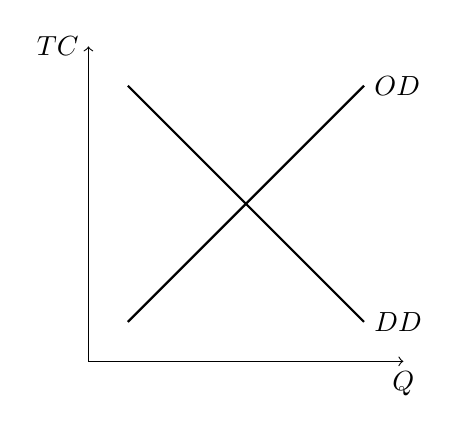
\begin{tikzpicture}
        \draw[->] (0,0) -- (0,4) node[left] {$TC$};
        \draw[->] (0,0) -- (4,0) node[below] {$Q$};
        \draw[thick] (0.5,3.5) -- (3.5,0.5) node[right] {$DD$};
        \draw[thick] (0.5,0.5) -- (3.5,3.5) node[right] {$OD$};
    \end{tikzpicture}
    \caption{Oferta y demanda de divisas}
\end{figure}

Cuando sube el tipo de cambio baja, y una \textit{devaluación} cuando el tipo de cambio sube. Dado que cuando se devalúa el tipo de cambio, las exportaciones aumentan y las importaciones disminuyen, mejorando los saldos exteriores de la economía. Ésta es la razón por la que se utiliza la devaluación como instrumento de ajuste por parte de las autoridades económicas. No obstante, la efectividad de este instrumento se produce, por lo general, tan sólo a corto plazo, ya que a largo plazo los precios también se ajustan y acaba compensándose la ventaja temporal lograda.

Además del \textit{tipo de cambio bilateral} también se utiliza ampliamente en la economía internacional el \textit{tipo de cambio efectivo}. Dicho tipo de cambio trata de fijar la evolución de una moneda (por ejemplo, el euro) en un periodo determinado respecto al conjunto de divisas con las que mantiene intercambios. Para ello se toma un año como base que sirva como nivel de referencia y se selecciona el conjunto de países respecto al cual se pretende estudiar la evolución de la moneda; cada país se introduce con una ponderación o peso según la importancia de los flujos comerciales existentes entre ambos países. El tipo de cambio resultante es un índice. Valores por encima de 100 indican que se está produciendo una depreciación de la moneda respecto al conjunto de monedas de referencia, mientras que valores por debajo de 100 serían un indicio de apreciación, cuando se utiliza la definición directa del tipo de cambio.

De esta forma, si el país $i$ mantiene relaciones comerciales con Estados Unidos, el Reino Unido, Japón, Suiza y otros países, su tipo de cambio efectivo vendrá dado por la siguiente expresión:

\[
TCE_i = [(TC_{id}/TC_{i0}) \times d + (TC_{il}/TC_{i0}) \times l + (TC_{iy}/TC_{i0}) \times y + (TC_{is}/TC_{i0}) \times fs + \ldots ] \times 100
\]

siendo $d, l, y$ y $fs$ las ponderaciones del dólar, libra, yen y franco suizo, respectivamente. Nótese que $(d + l + y + fs + \ldots) = 1$. Se puede también escribir de forma simplificada:

\[
TCE_i = \sum \left[ \left( \frac{TC_{ij}}{TC_{i0}} \right) \times p_j \right] \times 100
\]

donde $p_j$ son las ponderaciones, $TC_{ij}$ son los tipos de cambio bilaterales en el momento presente y $TC_{i0}$ representa los tipos de cambio bilaterales en el año base.

Asimismo, cabe diferenciar los \textit{tipos de cambio reales} de los \textit{nominales}. Los \textit{tipos de cambio nominales} son aquellos que establecen el precio de una moneda en términos de las demás monedas de la otra, mientras que los \textit{tipos de cambio reales} son los que se obtienen al ajustar el tipo de cambio nominal tomando en consideración algún índice de precios. Así, el \textit{tipo de cambio bilateral real} vendría dado por la fórmula siguiente:

\[
TCR = TC(P^*/P)
\]

siendo $P^*$ un índice de precios extranjeros y $P$ los precios nacionales equivalentes. Finalmente, el \textit{tipo de cambio efectivo real} puede definirse tal y como se presenta en la expresión siguiente:

\[
TCER_r = \sum \left( \frac{TCR_{ij}}{TCR_{j0}} \times p_j \right) \times 100
\]

\section*{TIPOS DE CAMBIO FLEXIBLES Y TIPOS DE CAMBIO FIJOS}

En los \textit{sistemas de tipos de cambio flexibles} los mercados de divisas son libres y el tipo de cambio fluctúa siguiendo los movimientos de la oferta y la demanda. A pesar de que las autoridades monetarias pueden intervenir ocasionalmente, no suele ser éste el caso y suelen dejar que el tipo de cambio se sitúe en el valor que determinen los mercados\footnote{Este es el régimen actualmente importante en el caso de la zona euro frente al resto del mundo. Dentro de la Unión Monetaria Europea no hay sino una moneda, el euro, por lo que el tipo de cambio no es un factor que, en la actualidad, afecte a una parte muy significativa del comercio comunitario, puesto que las transacciones intra-zona suponen aproximadamente el 50\% del total.}. Dichos mercados se ven afectados por las variables analizadas anteriormente y que no constituyen otra cosa sino los movimientos de la balanza de pagos, tanto en su vertiente de bienes y servicios como de capitales. Un desequilibrio de la balanza de pagos afectará al tipo de cambio, pero lo importante de este tipo de sistemas es que la variación ocasionada sobre el tipo de cambio llevará finalmente al reequilibrio de la balanza de pagos. Así, por ejemplo, se produce un aumento de las importaciones debido a que la renta europea es más elevada, ello provocará un déficit en la balanza de pagos. Este déficit desplazará a la derecha la demanda de divisas, por lo que será necesario hacer frente a más pagos por importaciones. El nuevo equilibrio del mercado de divisas se producirá con un tipo de cambio más alto, es decir, se producirá una depreciación del euro, posteriormente un aumento de las exportaciones y, finalmente, se volverá al equilibrio en la balanza de pagos. Por este motivo, en los regímenes de tipo de cambio flexibles la balanza de pagos siempre tenderá al equilibrio.

Por otro lado, en los \textit{sistemas de tipos de cambio fijos} las autoridades económicas intervienen en los mercados de divisas para limitar sus fluctuaciones. El banco central delimita el intervalo dentro del cual se sitúa el tipo de cambio oficial, dejando que éste fluctúe dentro de unos límites o bandas, definiéndose un \textit{tipo de cambio máximo} y uno \textit{mínimo}\footnote{De acuerdo con el Fondo Monetario Internacional, los regímenes de tipos de cambio fijos convencionales son aquéllos en que las monedas fluctúan en torno a una banda máxima de alrededor del 1\%. Cuando las bandas de fluctuación son más anchas, reciben el nombre de regímenes de tipos de cambio fijos dentro de bandas horizontales. La principal diferencia entre ambas es que, con una mayor amplitud de las bandas, existe un grado superior de discrecionalidad de la política monetaria.}. Dicho banco central tan sólo intervendrá cuando el mercado tienda a situar el tipo de cambio de equilibrio fuera de la banda.

El gráfico a) de la Figura 7.2 muestra una situación de equilibrio que coincide con el tipo de cambio central u oficial ($TC_c$). En el gráfico b), la moneda se encuentra apreciada, de forma que el equilibrio estaría fuera de la banda inferior. En ese caso, el banco emisor intervendrá vendiendo su moneda para que se deprecie y comprando a cambio la divisa respecto a la cual se ha apreciado. La cantidad de divisas que comprará es la distancia horizontal que separa la cantidad ofrecida ($Q_s$) de la cantidad demandada ($Q_d$) al precio dado por la banda inferior $TC_c$. De este modo, el banco emisor neutraliza el exceso de oferta (o la escasez de demanda). No tendrá ningún problema en vender la moneda nacional, pues lo hace a un precio más barato de lo que resultaría del equilibrio de mercado.

Si la situación fuera la inversa (depreciación de la moneda nacional respecto de la moneda extranjera), el banco central debería intervenir realizando la operación opuesta, es decir, vendiendo divisas a cambio de la moneda nacional. La cantidad vendida será la diferencia entre la cantidad demandada y la ofrecida al precio de la banda superior. Así, se neutraliza el exceso de demanda existente (o la escasez de oferta) al precio $TC_s$.

\begin{figure}[h]
    \centering
    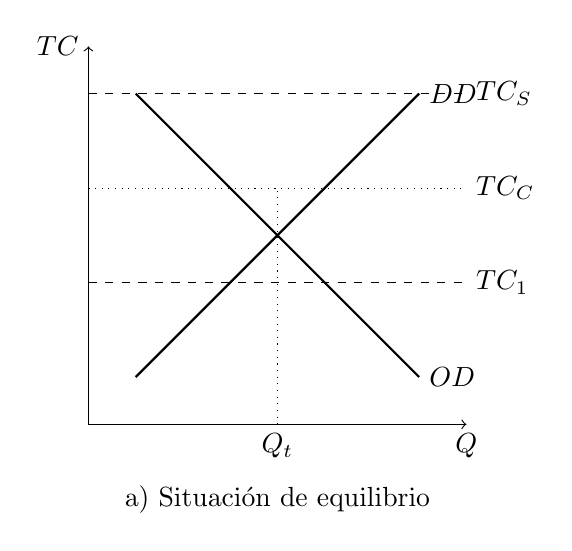
\begin{tikzpicture}[scale=1.2]
        % Ejes
        \draw[->] (0,0) -- (0,4) node[left] {$TC$};
        \draw[->] (0,0) -- (4,0) node[below] {$Q$};
        % Líneas horizontales
        \draw[dashed] (0,3.5) -- (4,3.5) node[right] {$TC_S$};
        \draw[dotted] (0,2.5) -- (4,2.5) node[right] {$TC_C$};
        \draw[dashed] (0,1.5) -- (4,1.5) node[right] {$TC_1$};
        % Oferta y demanda
        \draw[thick] (0.5,3.5) -- (3.5,0.5) node[right] {$OD$};
        \draw[thick] (0.5,0.5) -- (3.5,3.5) node[right] {$DD$};
        % Equilibrio
        \draw[dotted] (2,0) -- (2,2.5);
        \node[below] at (2,0) {$Q_t$};
        % Etiqueta
        \node at (2,-0.8) {a) Situación de equilibrio};
    \end{tikzpicture}
    \hspace{1cm}
    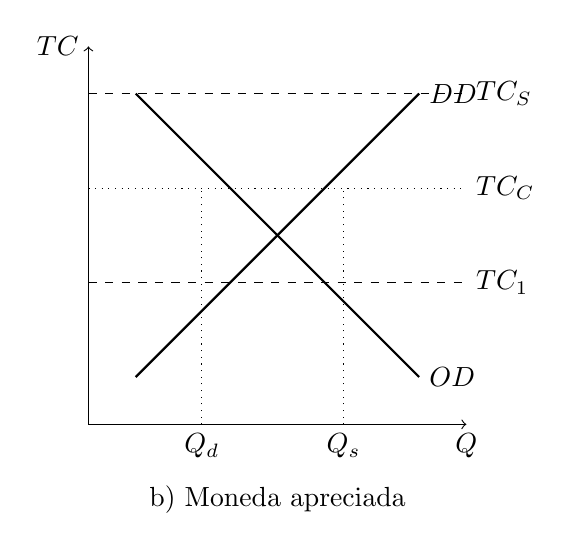
\begin{tikzpicture}[scale=1.2]
        % Ejes
        \draw[->] (0,0) -- (0,4) node[left] {$TC$};
        \draw[->] (0,0) -- (4,0) node[below] {$Q$};
        % Líneas horizontales
        \draw[dashed] (0,3.5) -- (4,3.5) node[right] {$TC_S$};
        \draw[dotted] (0,2.5) -- (4,2.5) node[right] {$TC_C$};
        \draw[dashed] (0,1.5) -- (4,1.5) node[right] {$TC_1$};
        % Oferta y demanda
        \draw[thick] (0.5,3.5) -- (3.5,0.5) node[right] {$OD$};
        \draw[thick] (0.5,0.5) -- (3.5,3.5) node[right] {$DD$};
        % Equilibrio fuera de la banda
        \draw[dotted] (1.2,0) -- (1.2,2.5);
        \node[below] at (1.2,0) {$Q_d$};
        \draw[dotted] (2.7,0) -- (2.7,2.5);
        \node[below] at (2.7,0) {$Q_s$};
        % Etiqueta
        \node at (2,-0.8) {b) Moneda apreciada};
    \end{tikzpicture}
    \caption{a) Situación de equilibrio \hspace{1cm} b) Moneda apreciada}
    \label{fig:tc-fijos}
\end{figure}

Puesto que las situaciones de apreciación o depreciación de una moneda siempre hay que contemplarlas en términos relativos (si una moneda se aprecia respecto de otra, la segunda se deprecia respecto de la primera), los bancos centrales, en el caso de los países integrantes del Sistema Monetario Europeo, acordaron intervenir de manera simultánea y de forma simétrica cuando se produjeran desequilibrios que situaran el tipo de cambio bilateral fuera de las bandas de fluctuación establecidas.

En cuanto a las ventajas e inconvenientes de adoptar un sistema de tipos de cambio fijos frente a un sistema flexible, ha existido tradicionalmente un amplio debate sobre cuál de los dos es mejor para el buen funcionamiento de la economía. Las ventajas que pueden esgrimirse a favor de los tipos de cambio fijos se refieren, fundamentalmente, a la estabilidad de los mismos proporcionan a los intercambios, tanto comerciales como de inversión (a pesar de la posibilidad siempre existente de utilizar formas de coberturas para evitar riesgos), así como el menor peligro de que el tipo de cambio sufra excesos de volatilidad o que, incluso, se sitúe en niveles excesivamente apreciados o depreciados. Sin embargo, a favor de los tipos de cambio flexibles puede decirse que, en ciertas circunstancias, puede ser un instrumento de política económica para equilibrar la balanza de pagos, evitando los costes de que dicho ajuste se realice en la parte real de la economía. Asimismo, en regímenes de tipos de cambio fijos pueden sufrirse ataques especulativos cuando los mercados entienden que el nivel de la moneda es demasiado apreciado, cosa que no ocurriría con tipos de cambio flexibles. Otro inconveniente de los tipos de cambio fijos es la dificultad que surge a la hora de elegir el tipo de cambio oficial, de modo que se sitúe lo más próximo posible al tipo de cambio de equilibrio.

En los años setenta se optó por los tipos de cambio flexibles como reacción a la mala experiencia derivada del funcionamiento del sistema de Bretton Woods. Sin embargo, como se verá en el tema siguiente, son muy variados los regímenes cambiarios actualmente imperantes en el mundo que se sitúan entre los dos extremos y que han intentado adaptarse a las condiciones económicas y a los objetivos de política monetaria en cada caso.

\section*{FORMAS DE MEDIR LA INTEGRACIÓN FINANCIERA INTERNACIONAL}

En la economía internacional existen un conjunto de paridades que implican ciertas relaciones de equilibrio entre las variables internas y las del resto del mundo, que a su vez sustentan las hipótesis básicas de los modelos de determinación del tipo de cambio. En un contexto de mercados financieros cada vez más integrados, los rendimientos de activos internacionales con características similares de riesgo deberían ser iguales. Por este motivo, todas las paridades que se van a describir a continuación se utilizan también como medida del grado de integración financiera alcanzada.

Feldstein y Horioka plantearon en 1980 una controversia, aún no zanjada, sobre lo que constituía, a su entender, una paradoja: a pesar de la liberalización de los mercados internacionales de capitales, la movilidad neta era reducida, pues el ahorro nacional se dedicaba básicamente a la financiación de la inversión nacional, los saldos netos de la balanza de pagos tienden al equilibrio y las transferencias netas estaban estancadas en términos del PIB. Por tanto, llegaron a la conclusión de que el mercado mundial de capitales seguía segmentado.

Posteriormente, Frankel (1993) rechazó la tesis anterior y afirmó que el grado de integración de los mercados ha crecido de forma significativa durante las dos últimas décadas. Para su medición propone cuatro definiciones de movilidad perfecta de capitales que son contrastables. Las tres primeras son lo que podría llamarse un \textit{enfoque preciso}, y se corresponden con diferentes definiciones de la paridad de intereses, mientras que la última es un \textit{enfoque cuantitativo} y consiste en el criterio de Feldstein y Horioka.

La \textit{paridad de intereses cubierta} implica que, en ausencia de riesgo de cambio, es decir, cuando existe cobertura a plazo, los flujos de capital tienden a igualar los tipos de interés nominales entre países. En el mercado de divisas a plazo se puede comprar y vender divisas en el futuro a un precio estipulado hoy. El tipo de cambio a plazo se denomina tipo de cambio \textit{forward} a un plazo determinado $T$ ($F_T$, que designaremos por $F$ para simplificar). Comparando dicha cotización a plazo con el tipo de cambio al contado ($TC$), también denominado tipo \textit{spot}, se puede conocer la apreciación o depreciación de la moneda cotizada por el mercado, lo que se conoce como prima a plazo (si la diferencia es positiva) o como descuento a plazo si la diferencia es negativa. La rentabilidad bruta de un inversor en activos internos, suponiendo que el plazo de vencimiento es de un año, viene dada por la siguiente expresión:

\[
RB = (1 + i)
\]

siendo $i$ el tipo de interés nacional. También puede invertir en activos externos comprando, con la moneda nacional, $1/TC$ unidades de moneda extranjera y luego invertirla en activos externos, obteniendo una rentabilidad bruta:

\[
RB^* = \frac{1}{TC} (1 + i^*)
\]

donde $i^*$ representa el tipo de interés extranjero.

A continuación, convierte los ingresos futuros en moneda nacional cubriéndose del riesgo en el mercado a plazo:

\[
RB^* = \frac{F}{TC} (1 + i^*)
\]

Si existiera perfecta movilidad de capitales, los rendimientos deberían igualarse:

\[
(1 + i) = \frac{F}{TC} (1 + i^*)
\tag{7.1}
\]

Por otra parte, designando por $D$ la variación del tipo de cambio, podemos escribir:

\[
D = \frac{F - TC}{TC}
\]

de donde $D = \frac{F}{TC} - 1$, $\frac{F}{TC} = D + 1$.

Sustituyendo $\frac{F}{TC}$ en la Ecuación (7.1) se tiene:

\[
(1 + i) = (D + 1)(1 + i^*)
\]
\[
1 + i = D + Di^* + 1 + i^*
\]
\[
i = D + Di^* + i^*
\]
\[
i - i^* = D + Di^*
\]

Como $Di^*$ tiende a cero, puede escribirse que

\[
i - i^* \approx D
\]

Es decir, la diferencia en los tipos de interés coincide con la apreciación/depreciación de la moneda.

\[
i - i^* = \frac{F - TC}{TC}
\tag{7.2}
\]

La expresión anterior equivale a:

\[
i = i^* + \frac{F - TC}{TC}
\]

donde $\frac{F - TC}{TC}$ mide el premio o descuento a plazo.

Si se desea tener en cuenta que los contratos \textit{forward} pueden realizarse a plazo inferior a un año, la Ecuación (7.2) quedaría de la forma siguiente:

\[
i - i^* = \frac{F - TC}{TC} \times \frac{360}{t}
\]

donde $t$ indica el número de días que restan hasta el vencimiento.

El premio o descuento \textit{forward} ($PF$), en porcentaje, se mediría como:

\[
PF = \frac{F - TC}{TC} \times \frac{360}{t} \times 100
\]

La \textit{paridad de intereses descubierta} establece que los mercados, en ausencia de trabas, tienden a igualar los tipos de interés para activos de riesgo similar entre países, incluso asumiendo el riesgo de cambio. El inversor conoce las rentabilidades, $i$ e $i^*$, y trabaja con las expectativas del mercado respecto a cuál será el tipo de cambio de la moneda. Las expresiones deducidas anteriormente son ahora válidas sin más que sustituir el tipo de cambio \textit{forward} ($F$) por el tipo de cambio esperado ($TC_e$):

\[
i - i^* = \frac{TC_e - TC}{TC}
\]

Finalmente, la teoría de la \textit{paridad de intereses reales} establece que los países deberían tener el mismo atipo de interés real (interés nominal menos tasa de inflación). Esta teoría se utiliza frecuentemente en modelos de determinación del tipo de cambio y considera que, a corto plazo, la depreciación esperada del tipo de cambio depende de las diferencias en el tipo de interés nominal pero que, a largo plazo, la variación del tipo de cambio vendrá determinada por las diferencias en la tasa de crecimiento de los precios (tasa de inflación):

\[
D = dP - dP^*
\]

$D$ = variación del tipo de cambio, $P$ = nivel de precios nacional, $P^*$ = nivel de precios del país extranjero.

Sustituyendo $D$ por $i - i^*$ y reordenando términos se obtiene que:

\[
i - dP = i^* - dP^*
\]

es decir, el tipo de interés real esperado en España debe ser igual al tipo de interés real esperado en el extranjero:

\[
r = r^*
\]

Ésta es la ecuación de Fisher internacional, según la cual los tipos de interés ex-ante deberían ser iguales a nivel internacional.

Finalmente, de acuerdo con \textit{la definición de Feldstein-Horioka}, si los movimientos de capitales son importantes, en un mundo globalizado e integrado no debería haber razones que justifiquen una correlación estrecha entre las tasas de ahorro e inversión nacionales. Sin embargo, de su trabajo empírico se desprendió el resultado contrario, lo que les llevó a formularla en términos de una paradoja. Su resolución se ha planteado desde dos ámbitos. Por un lado, desde el punto de vista de la segmentación, entre ambas variables existe una relación estructural, derivada de la restricción presupuestaria del gobierno. Por otro, se considera que no es una medida adecuada de la integración o de la movilidad de capitales, por lo que el análisis de las demás paridades internacionales sería una alternativa más conveniente.

Junto con estas paridades, referidas a los tipos de interés y, en general, a la integración de los mercados de capitales, la \textit{paridad del poder adquisitivo} (o \textit{PPA}) puede utilizarse como medida de la integración de los mercados de bienes a nivel internacional, hipótesis que, dado el elevado grado de apertura comercial de los países industrializados, debería, en principio, verificarse. La PPA puede considerarse la generalización de \textit{la ley de precio único}, según la cual, un bien debería tener el mismo precio en todos los países, una vez convertido a moneda común. El ejemplo del «Big Mac» es paradigmático y demuestra que esta proposición no tiende a verificarse en la realidad. La PPA, en su llamada \textit{versión absoluta}, se formularía en términos de índices de precios, de manera que:

\[
P = P^*TC
\]

aunque también se ha presentado en términos del tipo de cambio:

\[
TC = P/P^*
\]

que establecería que el tipo de cambio entre las monedas de dos países es igual al cociente de sus niveles generales de precios.

Por último, también se ha formulado tradicionalmente el concepto de \textit{PPA relativa}, al expresar la ecuación anterior en tasas de variación, tomando logaritmos y diferencias\footnote{Actualmente no se considera del todo correcta esta versión, a pesar de que puede resultar didáctica. Sería más adecuado formular la PPA relativa de la manera siguiente: $TC = kP/P^*$, introduciendo un factor $k$ que permite desviaciones del tipo de cambio nominal respecto a la ratio $P/P^*$.} De esta manera, la variación esperada del tipo de cambio entre dos monedas estaría reflejando las diferencias en tasas de inflación entre los dos países implicados, donde $dtc$, $dp$ y $dp^*$ representan las variaciones porcentuales de las variables:

\[
dtc = dp - dp^*
\]
